\subsection{Population Generator}
\begin{center}
    \textit{Terrain, Population markers} $\rightarrow$ \textbf{PopulationGenerator} $\rightarrow$ \textit{Population map} 
\end{center}
This generator will from the generated terrain, and the user-specified markers create an intensity map representing the population density for the world.
The intensity map is generated by first applying a few simplex noise layer that represents random distributions of populations throughout the world. 
Then a circle that fades in intensity along its border is added for each population marker. 
The terrain parameter is used to mask away certain locations from being inhabited e.g. oceans and tall mountain peeks.
This will be useful when generating the roads and specifying the blocks from the roads. 
In some places within the world, there is a larger need for higher buildings with many apartments. 
Some other places are more suitable for supermarkets or villas. 
The population map will be the backbone and a large factor for these generations. 

\begin{figure}[h]
  \centering
  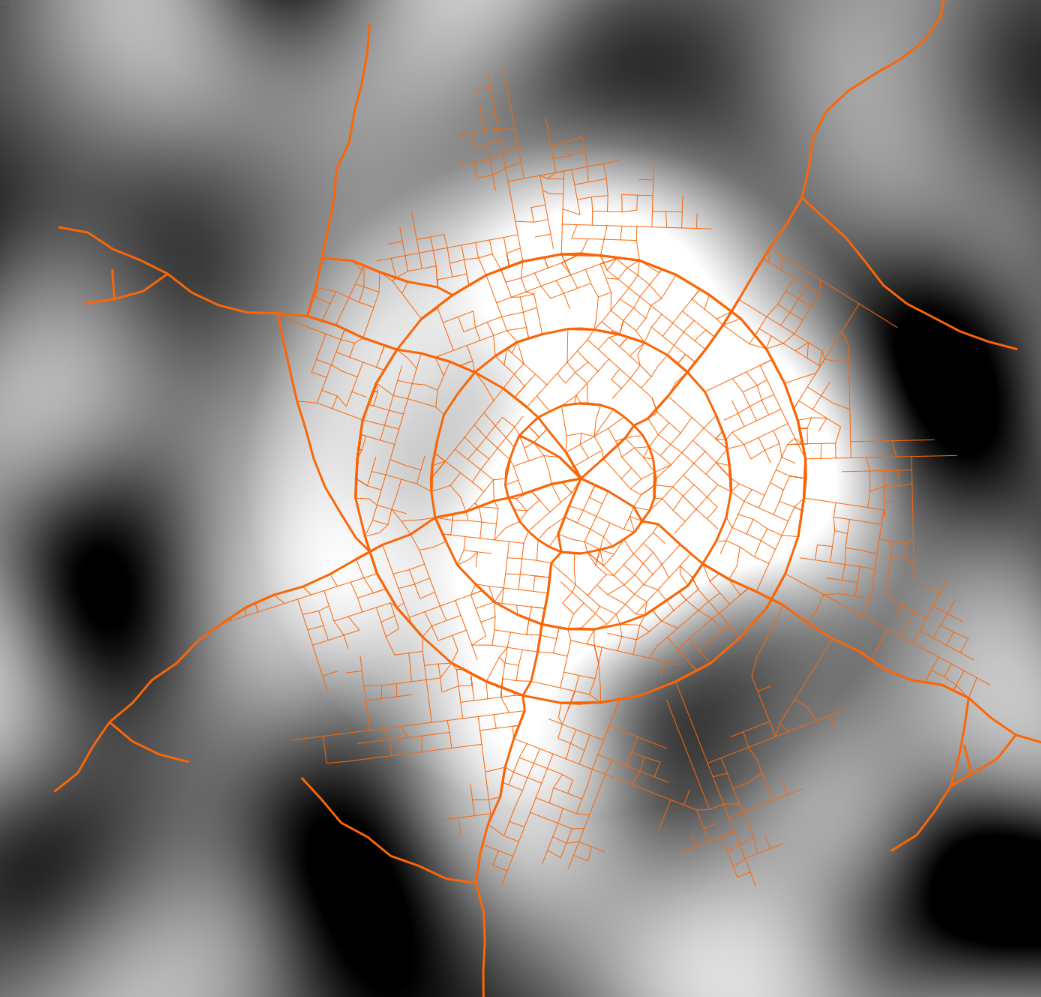
\includegraphics[width=0.6\textwidth]{figure/gen_population_map.png}
  \caption{An example of a population map with a Paris city generated within it}
  \label{fig:gen_population_map_example}
\end{figure}
